\documentclass[conference]{IEEEtran}
\makeatletter
\def\ps@headings{%
\def\@oddhead{\mbox{}\scriptsize\rightmark \hfil \thepage}%
\def\@evenhead{\scriptsize\thepage \hfil \leftmark\mbox{}}%
\def\@oddfoot{}%
\def\@evenfoot{}}
\makeatother
\pagestyle{headings}

\newcommand{\thetitle}{On the Linear Structure of Network Traffic: Predicting Flow Behavior}

%!TEX root = paper.tex

\usepackage[labelfont=bf,small]{caption}
\usepackage[font=small,labelfont=bf,position=top,nearskip=0em]{subfig}
\usepackage{cite,amsmath,amssymb,rotating,multirow,bigstrut,url,wrapfig,relsize,paralist,array,mathtools,units}
\usepackage[hyperfigures,bookmarks,bookmarksopen,bookmarksnumbered,colorlinks,linkcolor=black,citecolor=black,filecolor=blue,menucolor=black,pagecolor=blue,frenchlinks=true,pdftitle={\thetitle}]{hyperref}

%!TEX root = paper.tex

%% LABELING COMMANDS
\renewcommand{\sec}[1]{\label{sec:#1}}
\newcommand{\eqn}[1]{\label{eqn:#1}}
\newcommand{\fig}[1]{\label{fig:#1}}
\newcommand{\tab}[1]{\label{tab:#1}}
\newcommand{\thm}[1]{\label{thm:#1}}
\newcommand{\defn}[1]{\label{def:#1}}

%% REFERENCING COMMANDS
\newcommand{\Appendix}[1]{\hyperref[sec:#1]{Appendix~\ref*{sec:#1}}}
\newcommand{\Section}[1]{\hyperref[sec:#1]{Section~\ref*{sec:#1}}}
\newcommand{\Equation}[1]{\hyperref[eqn:#1]{Equation~\ref*{eqn:#1}}}
\newcommand{\Figure}[1]{\hyperref[fig:#1]{Figure~\ref*{fig:#1}}}
\newcommand{\Table}[1]{\hyperref[tab:#1]{Table~\ref*{tab:#1}}}
\newcommand{\Theorem}[1]{\hyperref[thm:#1]{Theorem~\ref*{thm:#1}}}
\newcommand{\Definition}[1]{\hyperref[def:#1]{Definition~\ref*{def:#1}}}

%% MATHEMATICAL NOTATIONS

% common algebraic domains
\newcommand{\N}{\mathbb{N}}
\newcommand{\Z}{\mathbb{Z}}
\newcommand{\Q}{\mathbb{Q}}
\newcommand{\R}{\mathbb{R}}

% standard operators & functors
\renewcommand{\Pr}{\mathrm{Pr}}
\newcommand{\Image}{\text{Im}}
\newcommand{\Kernel}{\text{Ker}}

% common constructs
\newcommand{\abs}[1]{{\left|#1\right|}}
\newcommand{\absx}[1]{{|#1|}}
\newcommand{\card}[1]{{\left|#1\right|}}
\newcommand{\cardx}[1]{{|#1|}}
\newcommand{\norm}[1]{{\lVert#1\rVert}}
\newcommand{\normx}[1]{{\Vert#1\Vert}}
\newcommand{\set}[1]{{\left\{#1\right\}}}
\newcommand{\setx}[1]{{\{#1\}}}
\newcommand{\parens}[1]{{\left(#1\right)}}
\newcommand{\parensx}[1]{{(#1)}}
\newcommand{\bracket}[1]{{\left[#1\right]}}
\newcommand{\bracketx}[1]{{[#1]}}
\newcommand{\seq}[1]{{\left<#1\right>}}
\newcommand{\seqx}[1]{{\lvert#1\rvert}}
\newcommand{\tuple}[1]{{\left<#1\right>}}
\newcommand{\tuplex}[1]{{\lvert#1\rvert}}
\newcommand{\floor}[1]{{\left\lfloor#1\right\rfloor}}
\newcommand{\floorx}[1]{{\lfloor#1\rfloor}}
\newcommand{\ceil}[1]{{\left\lceil#1\right\rceil}}
\newcommand{\ceilx}[1]{{\lceil#1\rceil}}
\newcommand{\round}[1]{{\left[#1\right]}}
\newcommand{\roundx}[1]{{[#1]}}
\newcommand{\fracx}[2]{{#1/#2}}
\newcommand{\fracp}[2]{{\left(\frac{#1}{#2}\right)}}
\newcommand{\fracpx}[2]{{(#1/#2)}}
\newcommand{\smallfrac}[2]{{\textstyle{\frac{#1}{#2}}}}

% standard notations
\newcommand{\trans}[1]{{#1}^T}
\newcommand{\inner}[2]{{#1}\trans{#2}}
\newcommand{\cross}{\times}
\newcommand{\tensor}{\otimes}
\newcommand{\directsum}{\oplus}
\newcommand{\iso}{\cong}
\newcommand{\union}{\cup}
\newcommand{\inter}{\cap}
\newcommand{\disunion}{\sqcup}
\newcommand{\Union}{\bigcup}
\newcommand{\Inter}{\bigcap}
\newcommand{\Disunion}{\bigsqcup}
\newcommand{\conj}{\wedge}
\newcommand{\disj}{\vee}
\newcommand{\Conj}{\bigwedge}
\newcommand{\Disj}{\bigvee}
\newcommand{\defeq}{=}
\renewcommand{\emptyset}{\varnothing}
\renewcommand{\setminus}{\,\raisebox{1pt}{$\smallsetminus$}\,}
\newcommand{\eldiv}{\,./\,}
\newcommand{\diag}{\text{diag}}
\newcommand{\rs}{\text{rs}}
\newcommand{\argmin}{\text{arg min}}

%% FORMATTING BEHAVIORS
\newcommand{\caps}[1]{{\small{#1}}}
\newcommand{\latin}[1]{\textit{#1}}
\newcommand{\defterm}[1]{\textit{#1}}
\newcommand{\newfootnote}[2]{\newcommand{#1}{\footnote{#2} }}
\renewcommand{\bullet}{\raisebox{2pt}{$\centerdot$}}
\renewcommand{\arraystretch}{1.3}

%% MISCELLANEOUS

\renewcommand{\vec}[1]{\mathbf{#1}}


\title{\vspace{-0.25em}\thetitle}
\author{
{\large{Stefan~Karpinski, John~R.~Gilbert, Elizabeth~M.~Belding}} \vspace{0.25em}\\
Department of Computer Science \\
University of California, Santa Barbara \vspace{0.35em}\\
\textit{\{sgk,gilbert,ebelding\}@cs.ucsb.edu}
}

\bibliographystyle{IEEEtran}

\newcommand{\figurename}{Figure}
\newcommand{\tablename}{Table}

\begin{document}
\maketitle

\begin{abstract}
We have observed that when network traffic behaviors are embedded into vector spaces in certain ways, they tend to exhibit a great deal of low-rank linear structure.
This observation leads us to the hypothesis that flow behaviors follow a specific type of finite mixture model.
Aside from being of theoretical interest, this model has practical consequences:
it allows us, among other things, to make detailed predictions about the probabilities of various future flow behaviors after observing only a handful of a flow's initial packets.
This practical application serves a dual function.
It provides a highly useful tool of network management, especially in wireless networks where such predictions can be leveraged to better allocate scarce bandwidth resources.
However, it also provides evidence that the hypothesized model not only explains the observed linear structure, but is an accurate model of real network traffic.
\end{abstract}

\section{Introduction}\sec{introduction}

\newfootnote{\flownote}{We use the common definition of a \textit{flow} as a sequence of packets sharing the same  ``5-tuple'': IP protocol type, source and destination nodes, and TCP/UDP port numbers.}

This paper is the first in a three-part series employing a numerical linear algebra techniques to understand and analyze network traffic patterns at a detailed level of individual flows and packets.\flownote
All three papers employ the same theoretical framework but investigate different fundamental applications of traffic modeling:
prediction, classification and generation.
In this paper we first present the framework and then demonstrate how it can predict the behavior of individual flows from the observation of only a handful of their initial packets.
% The following papers will focus on classification of flows according to application type and realistic workload generation.

The fundamental concept underlying this work is \emph{linear representation of network traffic}~\cite{Karpinski08}.
A linear representation is a function that maps sets of flows to vectors, the coordinates of which describe aspects of flow behavior;
it must distribute additively over set unions.
% the representation must also satisfy a simple linearity condition which we will describe in detail later.
% the sum of the representations of a set of flows is a vector that represents the aggregate behavior of the set of flows.
An entire traffic trace may be represented as a matrix whose rows are the representations of flows in the trace.
We restrict our consideration to a particularly natural and powerful class of representations whose coordinates are the frequencies of flow features in a set of flows.
For example, the representation can have a dimension for each packet size up to the maximum transfer unit (\caps{MTU});
coordinates in these dimensions indicate the count of packets of each size.
Port numbers, \caps{IP} protocol type, and inter-packet intervals can be handled similarly.
% Examples of flow features are the number of packets of a certain size or the use of a particular port number.
% The fundamental premise of this work, and of the sequel, is that the representatives of actual flow behaviors can be understood as being sampled from 

The essential observation of this research is that under such representations, real flows tend to lie near a small set of low-rank subspaces.
This property allows us to perform a drastic model reduction on trace traffic patterns while preserving the essential characteristics of the original traffic.
Moreover, when observable characteristics of flows are separated from features to be predicted, this model reduction is similar to a classical linear regression:
it allows us to use a least squares optimization on observed features to predict behavior.
We use this technique to predict the following characteristics of each flow from observing only a handful of its initial packets:
\begin{enumerate}
  \item the distribution of packets sizes,
  \item the distribution of inter-packet intervals,
  \item the number of packets that will be in the flow.
\end{enumerate}
From these properties we can indirectly predict many other properties, including the total duration and data volume.

At this point, it may be wise to address what we mean here by prediction.
Brief reflection shows that one cannot hope to accurately predict the exact behavior of flows:
flow behavior is nondeterministic---flows may exhibit the same initial behavior but subsequently behave quite differently.
The best we can do then is to predict a \emph{distribution} of possible outcomes given the observed initial behavior.
When compared with a specific outcome, such a prediction cannot be said to be ``wrong'' or ``right.''
How then can one measure the quality of a predicted distribution of outcomes?
This subtle and difficult issue is central to our evaluation methodology.

% real-world network traces tend to have approximately low-rank representation matrices despite the potential rank of such matrices being very large.
% Moreover, most flows' vectors lie on only one of a few even lower rank subspaces.
% Moreover, the low-rank subspace near which real traffic lies can be decomposed into subspaces of even lower rank, with almost all flows lying in one of these subspaces.
% Typically, these smaller subspaces are one-dimensional, but in some cases they may have up to a dozen dimensions.

% the vast majority of observed flow behaviors in any given trace lie in one of a handful low-rank subspaces.
% These subspaces are mostly of rank one, but a few have dimensions as high as ten.

% Karpinski~\emph{et~al.}~\cite{Karpinski08} further observed that the simplifications commonly used in traffic modeling correspond to multiplication of traffic representation matrices by low-rank matrices, averaging over rows or columns.
% They demonstrated experimentally that such simplifications severely distort important behavioral properties of traffic traces;
% viewing these simplification as low-rank matrix transformations, this is unsurprising:
% most of the detail of the original traffic behavior is destroyed.
% It was suggested that matrix factorization provides an alternative and superior means of model reduction.

\section{Background \& Motivation}\sec{background}\sec{motivation}

\begin{figure*}[t]
\begin{center}
\subfloat[\footnotesize{DARTMOUTH}]{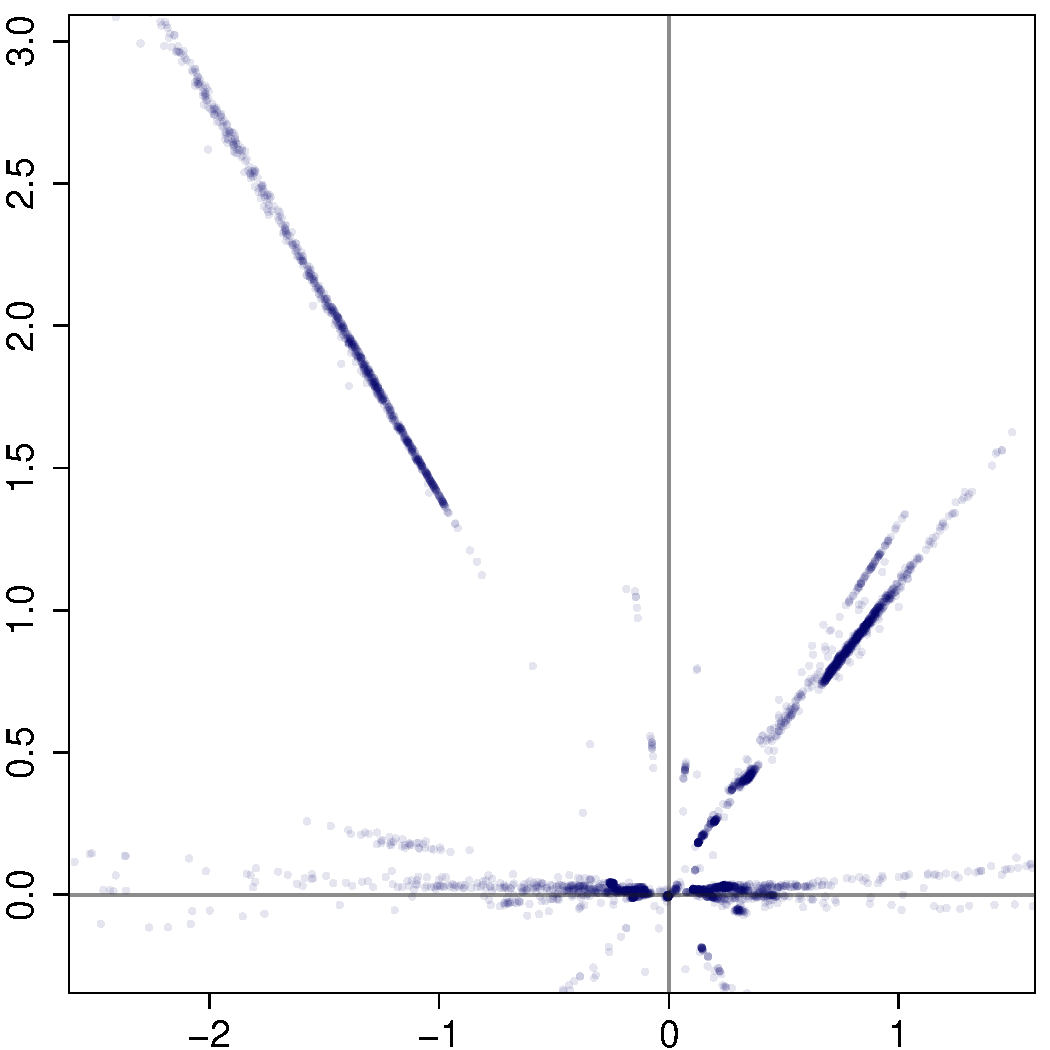
\includegraphics[width=1.15in]{svd/dart}}
\subfloat[\footnotesize{IETF 60}]{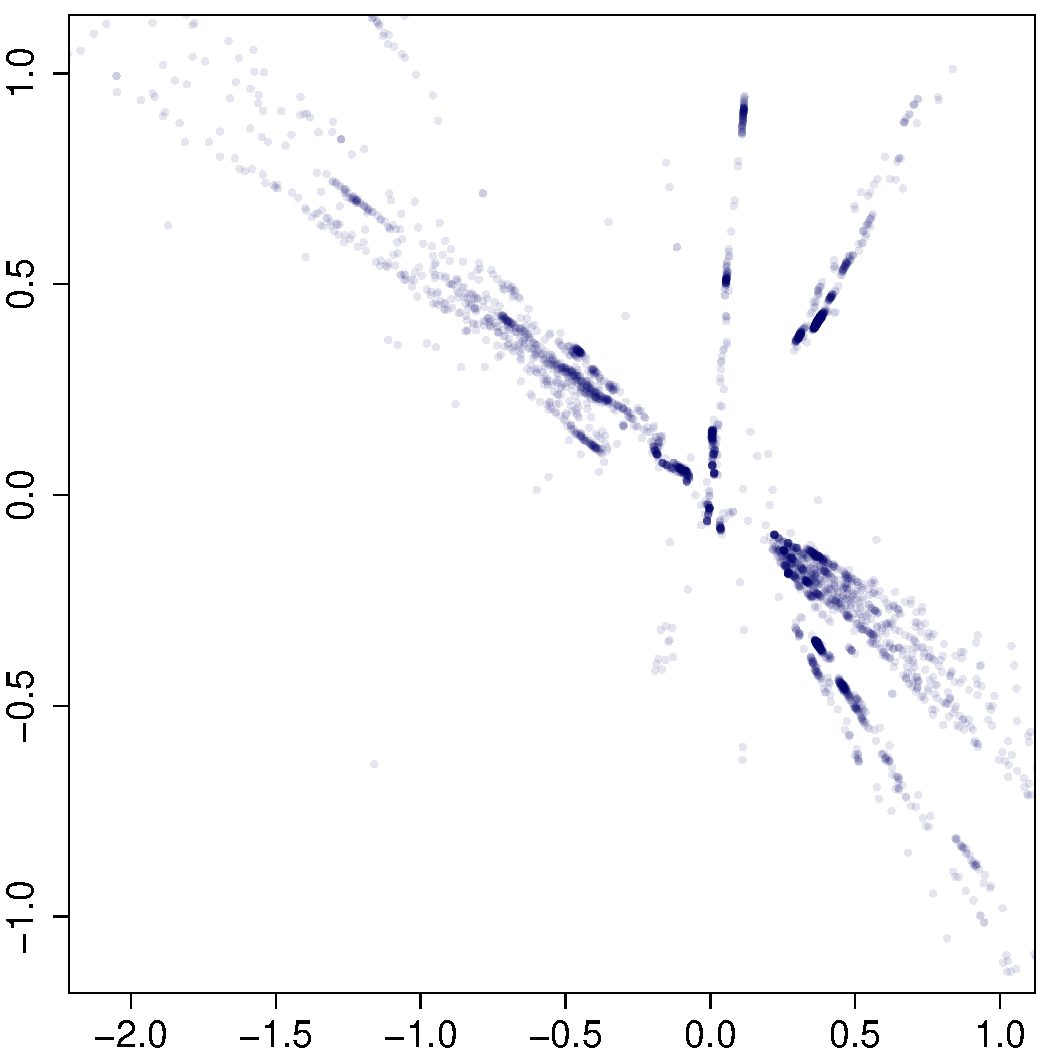
\includegraphics[width=1.15in]{svd/ie60}}
\subfloat[\footnotesize{IETF 67}]{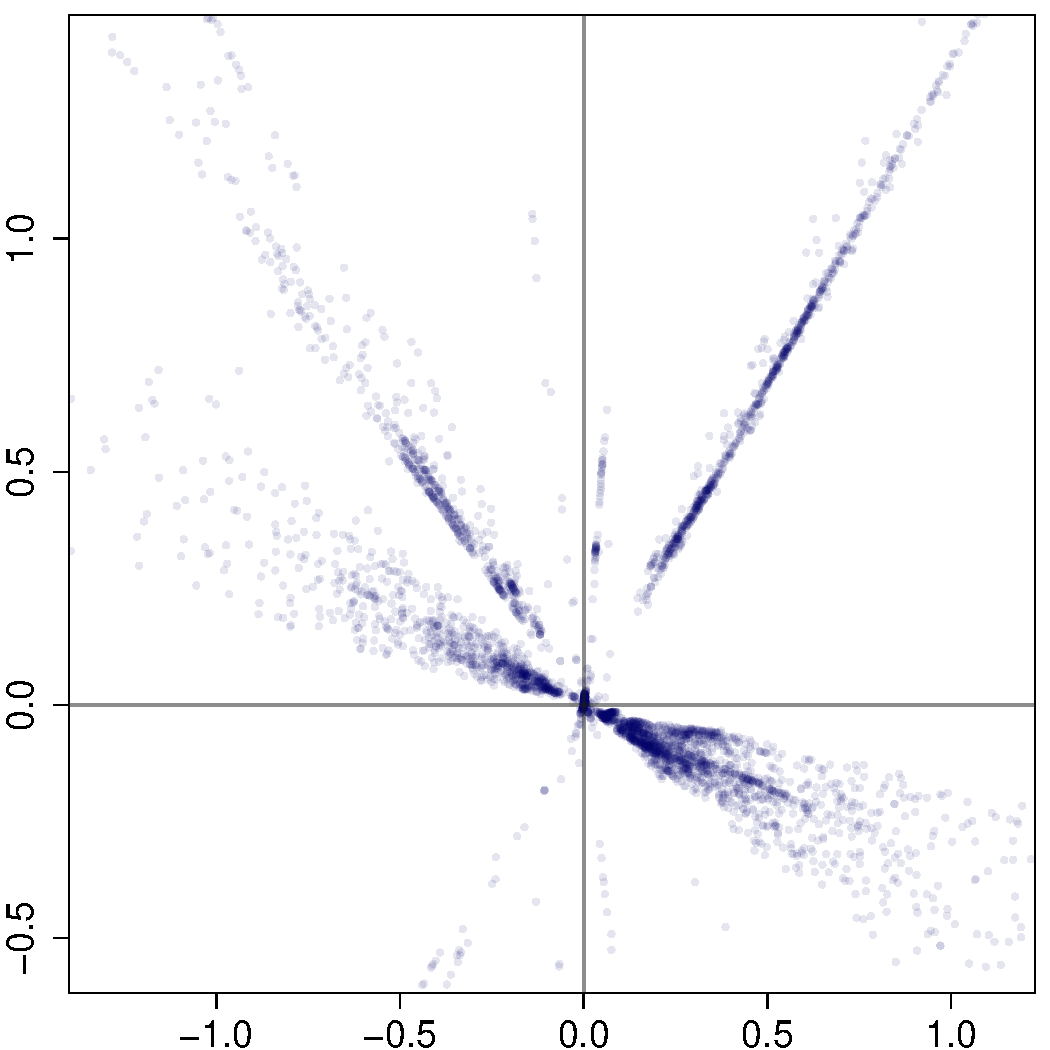
\includegraphics[width=1.15in]{svd/ie67}}
\subfloat[\footnotesize{SIGCOMM 2001}]{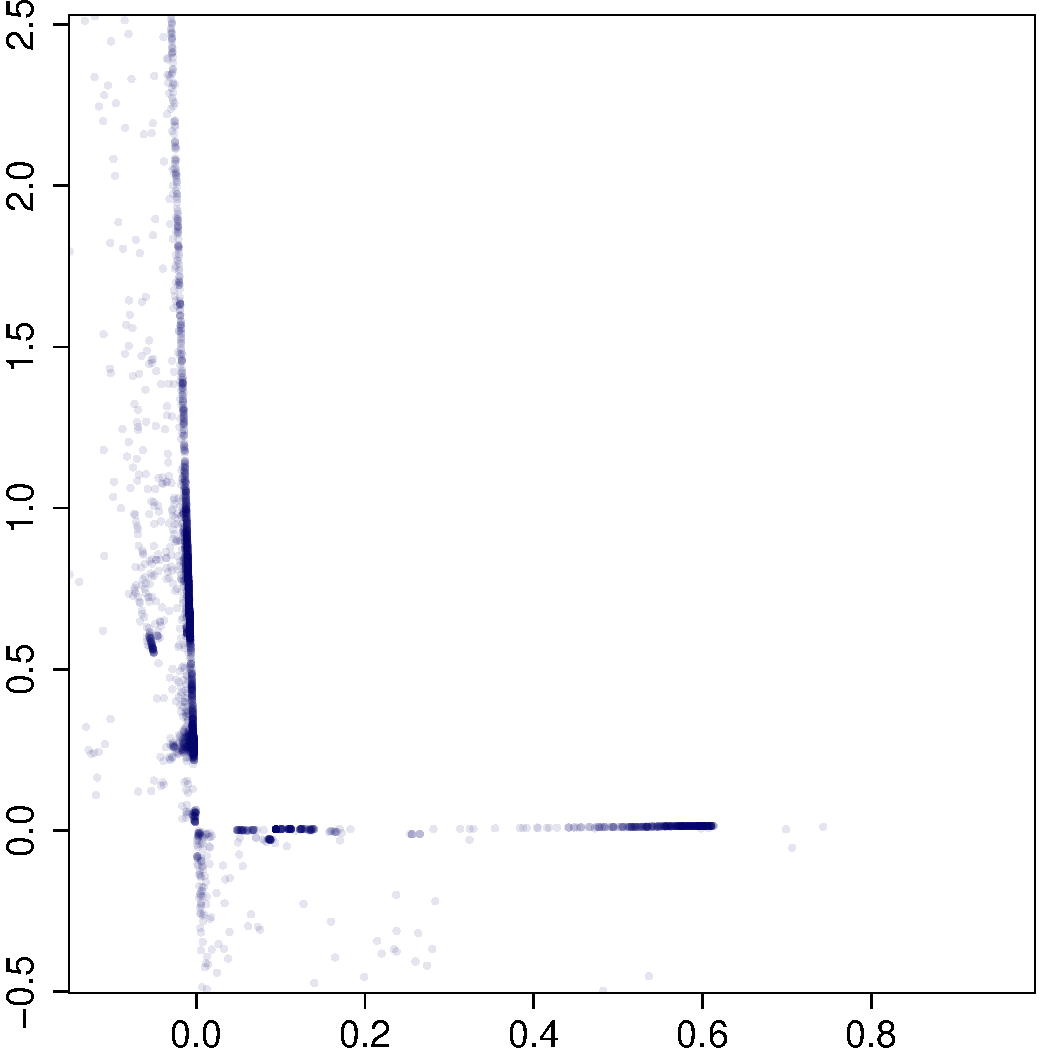
\includegraphics[width=1.15in]{svd/sc01}}
\subfloat[\footnotesize{SIGCOMM 2004}]{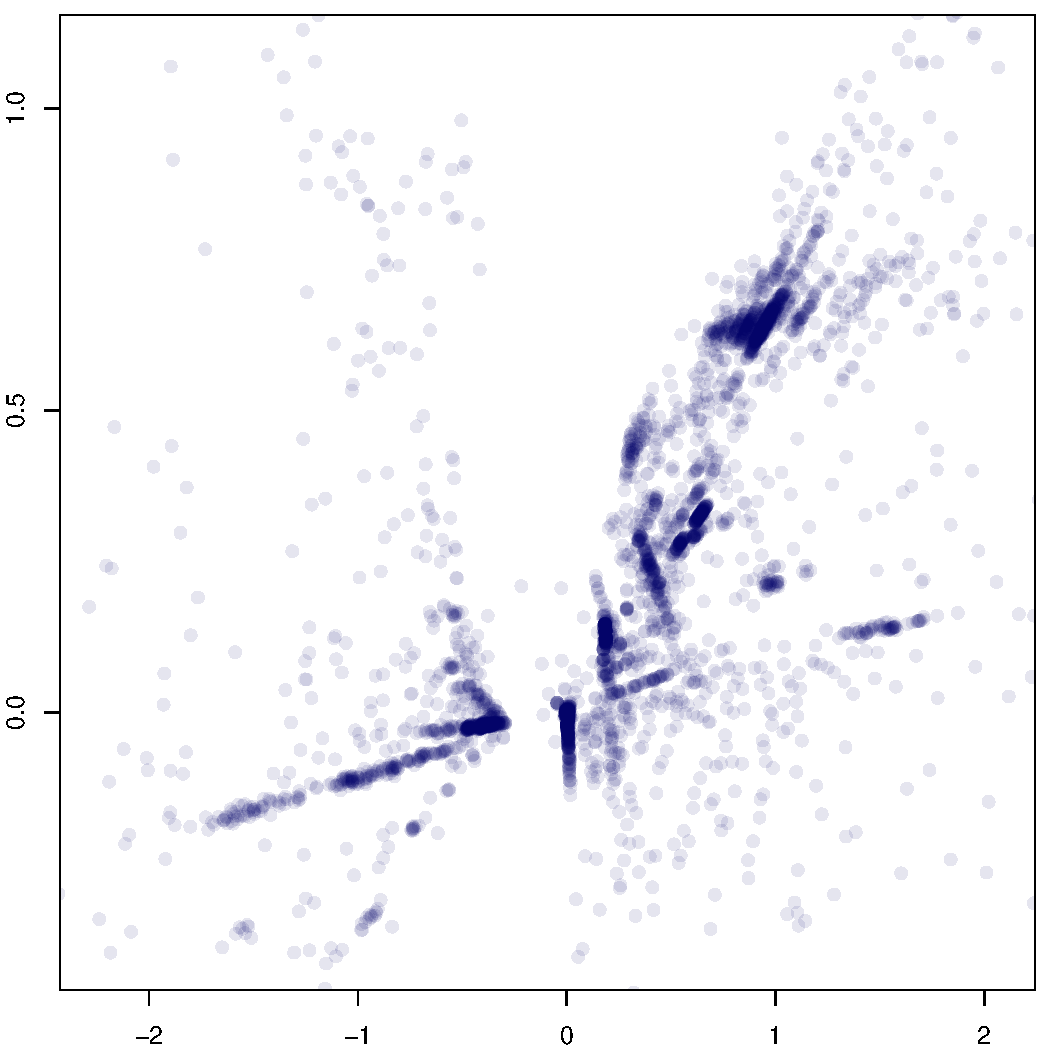
\includegraphics[width=1.15in]{svd/sc04}}
\subfloat[\footnotesize{UCSD}]{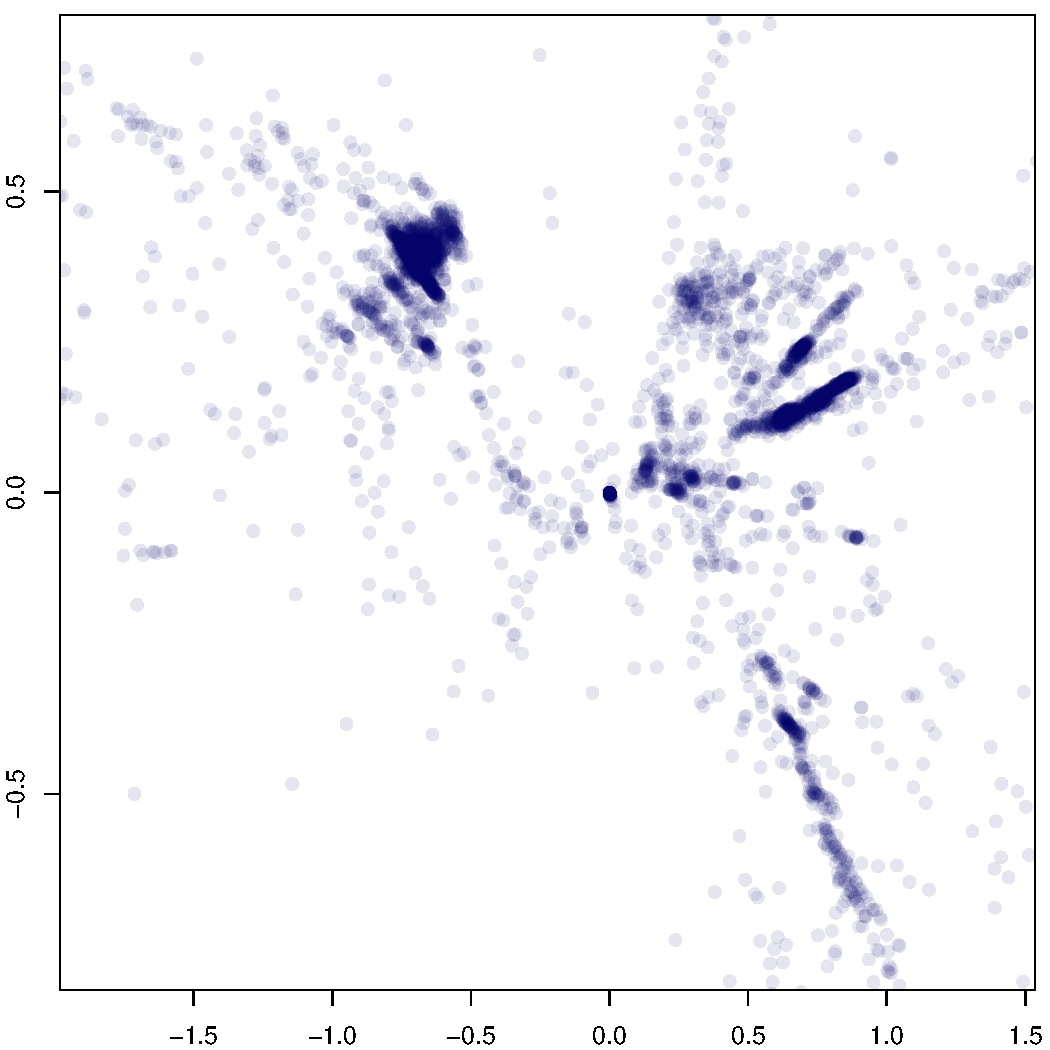
\includegraphics[width=1.15in]{svd/ucsd}}
\caption{SVD flow-behavior scatter plots for the six network traffic traces considered in this paper.} 
\fig{svd}
\end{center}
\vspace{-2em}
\end{figure*}

A linear representation, as proposed by Karpinski~\emph{et~al.}~\cite{Karpinski08}, maps sets of flows into a vector space such that disjoint union of sets becomes addition in the vector space:
\begin{align}
  \Phi(s_1 \disunion s_2) = \Phi(s_1) + \Phi(s_2).
\end{align}
The representation function should map each set of flows to a vector that in some sense describes their collective behavior.
For example: let $\Phi(s) \in \R^1$ be the number of packets in the flows in $s$.
Since the number of packets in the disjoint union of sets of flows is the sum of the number in each set individually, this representation is linear.
Given two representations, their direct sum is readily seen to also be a linear representation:
\begin{align}
  \Phi(s) = \Phi_1(s) \directsum \Phi_2(s).
\end{align}

A particularly powerful class of linear representations describes the behavior of collections of flows using histogram vectors to count the frequencies of various features.
A 1500-dimensional vector can be used to count the frequency of packet sizes seen, from one byte up to the typical \caps{MTU} of 1500 bytes.
In this representation, $\Phi(s)$ has as its $i$th entry the number of packets in $s$ of size $i$.
Since \caps{IP} protocols range from 0 to 255, the frequency of types in a set of flows can be represented in 256 dimensions.
Histogram representations for port numbers and inter-packet intervals are detailed in \Section{methodology}.
% Source and destination port numbers can similarly be represented using 65536-dimensional vectors.
% For practical purposes, however, this is too large a vector space, so we represent port numbers in 1000-dimensions, and reduce port numbers modulo 1000.
% Finally, we represent inter-packet intervals by first quantizing into 1500 bins of interval values as described by Karpinski~\emph{et~al.} and counting the number of intervals in flows occurring in each bin.
The representation we use is a direct sum of these histogram representations.
% The combination is a representation in 5256 dimensions.
An entire trace is represented as a matrix of such representation vectors---one flow per row.
This paper explores the linear structure of such matrices.

\newfootnote{\svdnote}{More precisely, the product of the first $k$ columns of $U$ with the first $k$ rows of $\trans{V}$ is a Frobenius-optimal rank-$k$ approximation of $X$.}

\newfootnote{\projectionnote}{We could normalize the vectors to unit length, but then our projection would be spherical, artificially introducing curvature into our visualization.}

To see the linear structure of these representation matrices, we apply one of the most powerful tools of linear algebra:
the singular value decomposition (\caps{SVD}).
This matrix decomposition can be applied to any real matrix, factoring it into a product of three real matrices:
\begin{align}
  X = US\trans{V}.
\end{align}
$U$ and $V$ are orthogonal and $S$ is diagonal, with entries of nonincreasing nonnegative value.
Among the useful properties of this factorization, is that the first $k$ columns of $US$ are an optimal $k$-dimensional reduced model of $X$.\svdnote
This property allows us to visualize the structure of $X$ using initial columns of $US$.
However, we are interested only interested in direction since
vectors differing only by magnitude lie in the same one-dimensional subspace.
To visualize direction while eliminating distance, we project all data points onto the unit-sum hyperplane from the origin.\projectionnote

\Figure{svd} illustrates the results of applying \caps{SVD} dimension reduction to sample matrices of six different traffic traces.
The figures show scatter plots of the most significant two projected \caps{SVD} coordinates for a matrix of 5000 sample flows from each trace.
% The original data encodes packet size distributions, inter-packet interval distributions, \caps{IP} protocol numbers, and port numbers for a sample of 5000 flows from each trace.
% The exact details of how the linear representation encodes these features will be discussed in \Section{methodology}.
Linear structure is visible in all six:
flow behaviors are heavily concentrated near low-dimensional subspaces.
Behaviors concentrated along a one-dimensional subspace appear as dark ``spots'' where many points have been plotted;
behaviors near two-dimensional subspaces appear as lines;
behaviors on higher-dimensional subspaces appear as ``smears.''
% There is a smattering of outliers, not especially near such structures.

The presence of linear structure in the matrix representations of several independent traffic traces immediately raises two significant questions.
The existential question: \emph{Why does this linear structure exist?}
Followed, of course, by the practical question: \emph{How can we exploit this structure?}
Neither question can be answered fully in a single paper, but we will begin to address the existential problem in the next section.
In the rest of the paper we apply this insight to the eminently practical problem of predicting the behavior of individual flows from the observation of only a few of their initial packets.

\section{Model \& Hypothesis}

Our answer to the question of why low-dimensional linear structure appears in the feature-frequency representation of network traffic can be expressed as a hypothetical model of flow behavior.
% A mixture model, to be specific.
We propose viewing each flow as having a probability distribution of possible behaviors it could exhibit.
% We propose that the behavior of each flow is drawn from a probability distribution on a space possible behaviors.
We hypothesize that the behavior distribution for most flows is a mixture of a relatively small set of ``basic behaviors.''
Moreover, only even smaller subsets of these basic behaviors are typically combined with each other.
Under these assumptions, we can express the distribution of each flow's behaviors as a finite mixture model~\cite{McLachlan00}:
\begin{align}\eqn{mixture-model}
  q_i(x) = \sum_{j=1}^r w_{ij} p_j(x),
\end{align}
Here $q_i$ and $p_j$ are probability density functions, and $w_{ij}$ are nonnegative weights, summing to unity for each $i$.
\Equation{mixture-model} is expressed succinctly as matrix multiplication.
Writing $Q_{ik} = q_i(k)$, $W_{ij} = w_{ij}$, and $P_{jk} = p_j(k)$, we have:
\begin{align}\eqn{mixture-model-matrix}
  Q = WP.
\end{align}
The number of basic behaviors, $r$, is the maximum possible rank of the feature distribution matrix, $Q$.
Moreover, we can partition the rows of $P$ into disjoint classes such that $w_{ij_1}$ and $w_{ij_2}$ are both non-zero only if $j_1$ and $j_2$ are in the same class.
Thus, each row of $Q$ is associated with exactly one class, and all the points associated with a class lie in the subspace spanned by its rows in $P$.

The properties of the model explain the structures seen in \Figure{svd}.
% This model is an ideal, and observed behaviors have noise introduced by sampling, imperfect adherence to the model, and outliers.
However, this is only one hypothesis that could fit the data.
Like any hypothesis, it must be tested.
The rest of this paper, aside from providing a practical application, serves as a hypothesis test:
we try to recover the matrices $W$ and $P$ from our imperfect observations of $Q$ and use the recovered model to predict real flow behaviors.
If the recovered model can make accurate predictions, this provides evidence that our model and hypothesis are largely accurate.

\section{Methodology}\sec{methodology}

\subsection{Linear Representation}\sec{linear-representation}

\subsection{Subspace Segmentation}\sec{subspace-segmentation}

\subsection{Subspace Factorization}\sec{subspace-factorization}

\subsection{Flow Behavior Prediction}\sec{flow-behavior-prediction}

\section{Results}\sec{results}

\section{Discussion}\sec{discussion}

\section{Conclusions}\sec{conclusions}

\bibliography{IEEE,references}

\end{document}
